\documentclass[border=5pt]{standalone}
% Shared by every figure. Colour marks the TYPE of a quantity, never decoration:
%   blue   (vec) equivariant: rotates with its fragment     -- solid arrows
%   orange (inv) invariant: unchanged by any rotation        -- dashed arrows
%   aqua   (att) attention / communication between elements
%   violet (out) what the network outputs
% Text is always ink; a coloured mark next to it carries the meaning.
\usepackage{amsmath,amssymb,bm}
\usepackage{tikz}
\usetikzlibrary{arrows.meta,positioning,fit,backgrounds,calc,shapes.geometric,
  shapes.misc,decorations.pathreplacing,decorations.pathmorphing,matrix,
  patterns,cd,shadows}
\definecolor{vec}{HTML}{2A78D6}
\definecolor{inv}{HTML}{EB6834}
\definecolor{att}{HTML}{1BAF7A}
\definecolor{out}{HTML}{4A3AA7}
\definecolor{ink}{HTML}{0B0B0B}
\definecolor{ink2}{HTML}{52514E}
\definecolor{ink3}{HTML}{8A877F}
\definecolor{neutral}{HTML}{F0EFEC}
\definecolor{rule}{HTML}{CFCCC4}
\definecolor{pieceA}{HTML}{E4E1DA}
\definecolor{pieceB}{HTML}{CDC9BF}
\definecolor{pieceC}{HTML}{B3AEA2}
\colorlet{vecfill}{vec!9}
\colorlet{invfill}{inv!10}
\colorlet{attfill}{att!11}
\colorlet{outfill}{out!9}
\tikzset{
  >={Stealth[length=2.3mm,width=1.7mm]},
  every picture/.style={line cap=round, line join=round},
  box/.style={draw=ink2, fill=neutral, rounded corners=2.5pt, align=center,
    font=\small, inner sep=4pt, minimum height=8mm, text=ink, line width=0.6pt, nohyph},
  vecbox/.style={box, draw=vec, fill=vecfill},
  invbox/.style={box, draw=inv, fill=invfill},
  attbox/.style={box, draw=att, fill=attfill},
  outbox/.style={box, draw=out, fill=outfill},
  plain/.style={box, draw=ink3, fill=white},
  arr/.style={->, draw=ink2, line width=0.7pt},
  vecarr/.style={->, draw=vec, line width=1.1pt},
  invarr/.style={->, draw=inv, line width=1.1pt, dash pattern=on 3.2pt off 1.8pt},
  attarr/.style={->, draw=att, line width=1.1pt, dash pattern=on 1.2pt off 1.4pt},
  outarr/.style={->, draw=out, line width=1.1pt},
  nohyph/.style={execute at begin node={\hyphenpenalty=10000\exhyphenpenalty=10000\relax}},
  lbl/.style={font=\footnotesize, text=ink2, align=center, nohyph},
  tlbl/.style={font=\footnotesize, text=ink, align=center, nohyph},
  group/.style={draw=ink3, dashed, rounded corners=5pt, inner sep=7pt},
  op/.style={circle, draw=ink2, fill=white, inner sep=0pt, minimum size=5.2mm,
    font=\small, line width=0.6pt},
  piece/.style={fill=#1, draw=none},
  intact/.style={draw=ink2, line width=0.6pt},
  fracture/.style={draw=ink, line width=1.5pt},
  token/.style={circle, fill=att, draw=white, line width=0.5pt, inner sep=0pt,
    minimum size=4.2pt},
  vtx/.style={circle, fill=ink, inner sep=0pt, minimum size=3pt},
  panel/.style={font=\small\bfseries, text=ink, anchor=north west},
}
% one piece of the cartoon, in its own centred frame: fill, intact edge, fracture edge
\newcommand{\drawpiece}[2]{% #1 = A|B|C, #2 = fill colour
  \fill[#2] \csname Piece#1\endcsname;
  \draw[intact] \csname Intact#1\endcsname;
  \draw[fracture] \csname Crack#1\endcsname;}
% a legend entry: a short line in a given style, then its text
\newcommand{\legendline}[3]{% #1 position, #2 style, #3 text
  \draw[#2] (#1) -- ++(0.7,0) node[right, tlbl, text=ink] {#3};}

% piece A: area 3.516, radius 1.322
\def\cAx{-1.129}\def\cAy{0.159}\def\rA{1.322}
\def\farAx{-0.317}\def\farAy{-1.283}
\def\PieceA{(0.583,1.175) -- (0.250,1.135) -- (-0.033,1.071) -- (-0.277,0.983) -- (-0.484,0.872) -- (-0.655,0.738) -- (-0.790,0.580) -- (-0.888,0.397) -- (-0.948,0.181) -- (-0.971,-0.109) -- (-0.955,-0.455) -- (-0.902,-0.679) -- (-0.810,-0.867) -- (-0.682,-1.029) -- (-0.518,-1.168) -- (-0.317,-1.283) -- (-0.100,-1.068) -- (0.240,-1.036) -- (0.392,-0.723) -- (0.645,-0.562) -- (0.933,-0.451) -- (1.179,-0.279) -- (1.051,-0.049) -- (0.927,0.183) -- (0.937,0.471) -- (0.859,0.722) -- (0.700,0.940) -- cycle}
\def\IntactA{(0.583,1.175) -- (0.250,1.135) -- (-0.033,1.071) -- (-0.277,0.983) -- (-0.484,0.872) -- (-0.655,0.738) -- (-0.790,0.580) -- (-0.888,0.397) -- (-0.948,0.181) -- (-0.971,-0.109) -- (-0.955,-0.455) -- (-0.902,-0.679) -- (-0.810,-0.867) -- (-0.682,-1.029) -- (-0.518,-1.168) -- (-0.317,-1.283)}
\def\CrackA{(-0.317,-1.283) -- (-0.100,-1.068) -- (0.240,-1.036) -- (0.392,-0.723) -- (0.645,-0.562) -- (0.933,-0.451) -- (1.179,-0.279) -- (1.051,-0.049) -- (0.927,0.183) -- (0.937,0.471) -- (0.859,0.722) -- (0.700,0.940) -- (0.583,1.175)}
\def\NameCracksA{\coordinate (A-0-0) at (0.583,1.175); \coordinate (A-1-0) at (-0.317,-1.283); \coordinate (A-1-1) at (-0.100,-1.068); \coordinate (A-1-2) at (0.240,-1.036); \coordinate (A-1-3) at (0.392,-0.723); \coordinate (A-1-4) at (0.645,-0.562); \coordinate (A-1-5) at (0.933,-0.451); \coordinate (A-1-6) at (1.179,-0.279); \coordinate (A-0-5) at (1.051,-0.049); \coordinate (A-0-4) at (0.927,0.183); \coordinate (A-0-3) at (0.937,0.471); \coordinate (A-0-2) at (0.859,0.722); \coordinate (A-0-1) at (0.700,0.940);}
\def\TokensA{-0.317/-1.283, 0.392/-0.723, 1.179/-0.279, 0.937/0.471, 0.583/1.175}
\def\TokenIdsA{1-0, 1-3, 1-6, 0-3, 0-0}
% piece B: area 2.203, radius 1.590
\def\cBx{0.124}\def\cBy{-0.872}\def\rB{1.590}
\def\farBx{-1.570}\def\farBy{-0.252}
\def\PieceB{(-1.570,-0.252) -- (-1.361,-0.335) -- (-1.123,-0.400) -- (-0.850,-0.445) -- (-0.528,-0.471) -- (-0.024,-0.478) -- (0.376,-0.466) -- (0.682,-0.434) -- (0.944,-0.384) -- (1.174,-0.314) -- (1.375,-0.226) -- (1.547,-0.119) -- (1.291,0.053) -- (1.029,0.212) -- (0.762,0.364) -- (0.472,0.472) -- (0.196,0.606) -- (-0.074,0.752) -- (-0.321,0.580) -- (-0.608,0.469) -- (-0.861,0.308) -- (-1.013,-0.005) -- (-1.353,-0.037) -- cycle}
\def\IntactB{(-1.570,-0.252) -- (-1.361,-0.335) -- (-1.123,-0.400) -- (-0.850,-0.445) -- (-0.528,-0.471) -- (-0.024,-0.478) -- (0.376,-0.466) -- (0.682,-0.434) -- (0.944,-0.384) -- (1.174,-0.314) -- (1.375,-0.226) -- (1.547,-0.119)}
\def\CrackB{(1.547,-0.119) -- (1.291,0.053) -- (1.029,0.212) -- (0.762,0.364) -- (0.472,0.472) -- (0.196,0.606) -- (-0.074,0.752) -- (-0.321,0.580) -- (-0.608,0.469) -- (-0.861,0.308) -- (-1.013,-0.005) -- (-1.353,-0.037) -- (-1.570,-0.252)}
\def\NameCracksB{\coordinate (B-1-0) at (-1.570,-0.252); \coordinate (B-2-0) at (1.547,-0.119); \coordinate (B-2-1) at (1.291,0.053); \coordinate (B-2-2) at (1.029,0.212); \coordinate (B-2-3) at (0.762,0.364); \coordinate (B-2-4) at (0.472,0.472); \coordinate (B-2-5) at (0.196,0.606); \coordinate (B-2-6) at (-0.074,0.752); \coordinate (B-1-5) at (-0.321,0.580); \coordinate (B-1-4) at (-0.608,0.469); \coordinate (B-1-3) at (-0.861,0.308); \coordinate (B-1-2) at (-1.013,-0.005); \coordinate (B-1-1) at (-1.353,-0.037);}
\def\TokensB{1.547/-0.119, 0.762/0.364, -0.074/0.752, -0.861/0.308, -1.570/-0.252}
\def\TokenIdsB{2-0, 2-3, 2-6, 1-3, 1-0}
% piece C: area 3.931, radius 1.785
\def\cCx{0.940}\def\cCy{0.345}\def\rC{1.785}
\def\farCx{-1.486}\def\farCy{0.989}
\def\PieceC{(0.731,-1.336) -- (0.902,-1.183) -- (1.030,-1.002) -- (1.115,-0.788) -- (1.156,-0.524) -- (1.153,-0.128) -- (1.106,0.127) -- (1.016,0.336) -- (0.882,0.514) -- (0.707,0.664) -- (0.489,0.787) -- (0.230,0.883) -- (-0.075,0.952) -- (-0.439,0.992) -- (-0.997,1.005) -- (-1.486,0.989) -- (-1.369,0.754) -- (-1.210,0.536) -- (-1.132,0.285) -- (-1.143,-0.002) -- (-1.018,-0.234) -- (-0.890,-0.465) -- (-0.620,-0.611) -- (-0.344,-0.745) -- (-0.054,-0.853) -- (0.213,-1.004) -- (0.476,-1.164) -- cycle}
\def\IntactC{(0.731,-1.336) -- (0.902,-1.183) -- (1.030,-1.002) -- (1.115,-0.788) -- (1.156,-0.524) -- (1.153,-0.128) -- (1.106,0.127) -- (1.016,0.336) -- (0.882,0.514) -- (0.707,0.664) -- (0.489,0.787) -- (0.230,0.883) -- (-0.075,0.952) -- (-0.439,0.992) -- (-0.997,1.005) -- (-1.486,0.989)}
\def\CrackC{(-1.486,0.989) -- (-1.369,0.754) -- (-1.210,0.536) -- (-1.132,0.285) -- (-1.143,-0.002) -- (-1.018,-0.234) -- (-0.890,-0.465) -- (-0.620,-0.611) -- (-0.344,-0.745) -- (-0.054,-0.853) -- (0.213,-1.004) -- (0.476,-1.164) -- (0.731,-1.336)}
\def\NameCracksC{\coordinate (C-2-0) at (0.731,-1.336); \coordinate (C-0-0) at (-1.486,0.989); \coordinate (C-0-1) at (-1.369,0.754); \coordinate (C-0-2) at (-1.210,0.536); \coordinate (C-0-3) at (-1.132,0.285); \coordinate (C-0-4) at (-1.143,-0.002); \coordinate (C-0-5) at (-1.018,-0.234); \coordinate (C-0-6) at (-0.890,-0.465); \coordinate (C-2-5) at (-0.620,-0.611); \coordinate (C-2-4) at (-0.344,-0.745); \coordinate (C-2-3) at (-0.054,-0.853); \coordinate (C-2-2) at (0.213,-1.004); \coordinate (C-2-1) at (0.476,-1.164);}
\def\TokensC{-1.486/0.989, -1.132/0.285, -0.890/-0.465, -0.054/-0.853, 0.731/-1.336}
\def\TokenIdsC{0-0, 0-3, 0-6, 2-3, 2-0}
\def\dScene{1.785}
\def\invd{0.5602}

\begin{document}
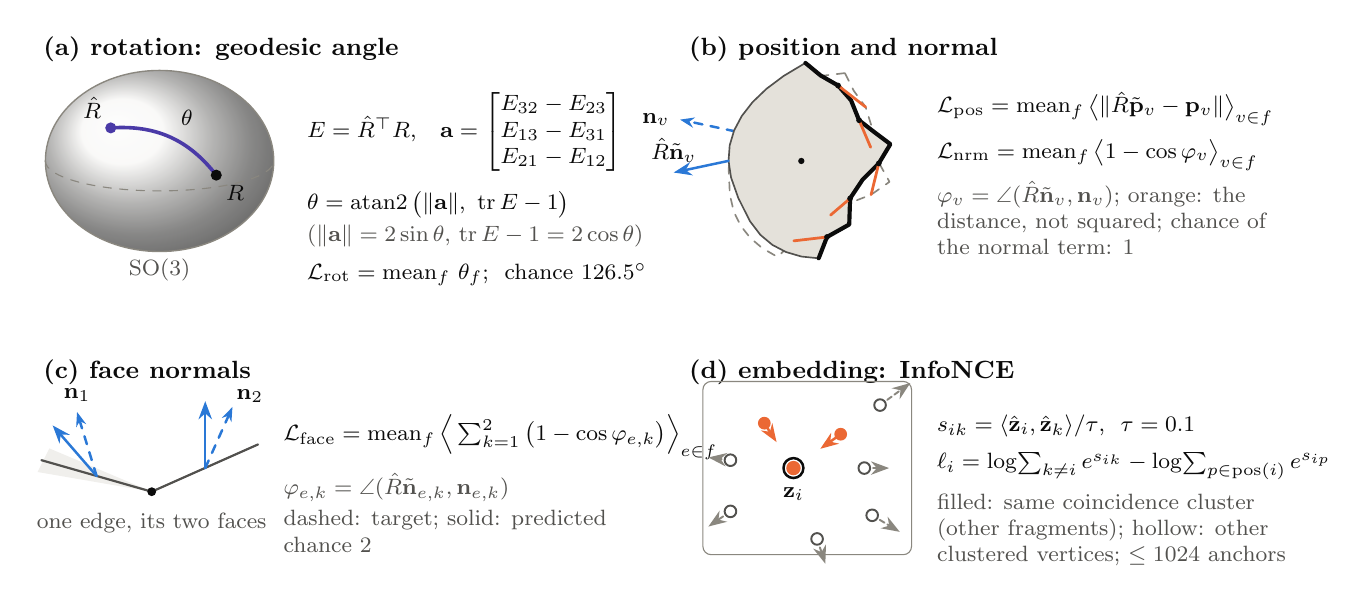
\begin{tikzpicture}
  \tikzset{form/.style={lbl, text=ink, anchor=north west, align=left}}
  % ===================== (a) rotation =====================
  \node[panel] at (-0.2,2.05) {(a) rotation: geodesic angle};
  \begin{scope}[shift={(1.4,0.35)}]
    \shade[ball color=neutral!60!white, opacity=0.9] (0,0) ellipse (1.45 and 1.15);
    \draw[ink3, line width=0.5pt] (0,0) ellipse (1.45 and 1.15);
    \draw[ink3, line width=0.4pt, dashed] (-1.45,0) arc[start angle=180, end angle=360, x radius=1.45, y radius=0.38];
    \coordinate (p) at (-0.62,0.42); \coordinate (q) at (0.72,-0.18);
    \draw[draw=out, line width=1.3pt] (p) to[bend left=28] node[midway, above right, tlbl] {$\theta$} (q);
    \fill[fill=out] (p) circle (2pt) node[above left, tlbl] {$\hat R$};
    \fill[ink] (q) circle (2pt) node[below right, tlbl] {$R$};
    \node[lbl] at (0,-1.38) {$\mathrm{SO}(3)$};
  \end{scope}
  \node[form] at (3.15,1.35) {$E=\hat R^{\top}R$,\quad $\mathbf a=\begin{bmatrix}E_{32}-E_{23}\\ E_{13}-E_{31}\\ E_{21}-E_{12}\end{bmatrix}$\\[6pt]
    $\theta=\operatorname{atan2}\big(\lVert\mathbf a\rVert,\ \operatorname{tr}E-1\big)$\\[2pt]
    {\color{ink2}($\lVert\mathbf a\rVert=2\sin\theta$, $\operatorname{tr}E-1=2\cos\theta$)}\\[4pt]
    $\mathcal L_{\mathrm{rot}}=\operatorname{mean}_f\,\theta_f$; \ chance $126.5^\circ$};

  % ===================== (b) position and normal =====================
  \node[panel] at (8.0,2.05) {(b) position and normal};
  \begin{scope}[shift={(9.55,0.35)}, scale=0.95]
    \begin{scope}[scale=1.0]
      \draw[ink3, dashed, line width=0.6pt] \PieceA;
      \NameCracksA
      \foreach \c/\k in {1/1,1/3,1/5,0/2,0/4}{\coordinate (T\c\k) at (A-\c-\k);}
      \coordinate (Tn) at (-0.888,0.397);
      \draw[vec, line width=0.9pt, dashed, -{Stealth[length=1.8mm,width=1.3mm]}] (Tn) -- ++(168:0.75) node[left, tlbl] {$\mathbf n_v$};
    \end{scope}
    \begin{scope}[rotate=24]
      \drawpiece{A}{pieceA}
      \NameCracksA
      \coordinate (Pn) at (-0.888,0.397);
      \draw[vecarr, line width=0.9pt] (Pn) -- ++(168:0.75) node[above, tlbl] {$\hat R\tilde{\mathbf n}_v$};
    \end{scope}
    \foreach \c/\k in {1/1,1/3,1/5,0/2,0/4}{
      \draw[inv, line width=1.0pt] (A-\c-\k) -- (T\c\k);
      \fill[ink] (A-\c-\k) circle (1.1pt);}
    \fill[ink] (0,0) circle (1.2pt);
  \end{scope}
  \node[form] at (11.15,1.35) {$\mathcal L_{\mathrm{pos}}=\operatorname{mean}_f\big\langle\lVert\hat R\tilde{\mathbf p}_v-\mathbf p_v\rVert\big\rangle_{v\in f}$\\[4pt]
    $\mathcal L_{\mathrm{nrm}}=\operatorname{mean}_f\big\langle 1-\cos\varphi_v\big\rangle_{v\in f}$\\[3pt]
    {\color{ink2}$\varphi_v=\angle(\hat R\tilde{\mathbf n}_v,\mathbf n_v)$; orange: the}\\ {\color{ink2}distance, not squared; chance of}\\ {\color{ink2}the normal term: 1}};

  % ===================== (c) face normals =====================
  \node[panel] at (-0.2,-2.05) {(c) face normals};
  \begin{scope}[shift={(1.3,-3.85)}]
    \coordinate (e) at (0,0);
    \fill[neutral] (e) -- (-1.3,0.55) -- (-1.45,0.25) -- cycle;
    \draw[ink2, line width=0.8pt] (-1.4,0.4) -- (e) -- (1.35,0.6);
    \fill[ink] (e) circle (1.6pt);
    % targets (dashed) and predictions (solid, rotated by the error)
    \draw[vec, line width=0.9pt, dashed, -{Stealth[length=1.8mm,width=1.3mm]}] (-0.7,0.2) -- ++(107:0.85) node[above, tlbl] {$\mathbf n_1$};
    \draw[vec, line width=0.9pt, dashed, -{Stealth[length=1.8mm,width=1.3mm]}] (0.68,0.3) -- ++(66:0.85) node[above right, tlbl, inner sep=1pt] {$\mathbf n_2$};
    \draw[vecarr, line width=0.9pt] (-0.7,0.2) -- ++(131:0.85);
    \draw[vecarr, line width=0.9pt] (0.68,0.3) -- ++(90:0.85);
    \node[lbl, anchor=north] at (0,-0.15) {one edge, its two faces};
  \end{scope}
  \node[form] at (2.85,-2.75) {$\mathcal L_{\mathrm{face}}=\operatorname{mean}_f\Big\langle\textstyle\sum_{k=1}^{2}\big(1-\cos\varphi_{e,k}\big)\Big\rangle_{e\in f}$\\[4pt]
    {\color{ink2}$\varphi_{e,k}=\angle(\hat R\tilde{\mathbf n}_{e,k},\mathbf n_{e,k})$}\\[2pt]
    {\color{ink2}dashed: target; solid: predicted}\\ {\color{ink2}chance 2}};

  % ===================== (d) correspondence embedding =====================
  \node[panel] at (8.0,-2.05) {(d) embedding: InfoNCE};
  \begin{scope}[shift={(9.5,-3.6)}]
    \draw[ink3, line width=0.4pt, rounded corners=3pt] (-1.2,-1.05) rectangle (1.45,1.15);
    \coordinate (zi) at (-0.05,0.05);
    \foreach \x/\y in {0.55/0.48,-0.42/0.62}{
      \draw[inv, line width=0.9pt, ->, shorten >=2.5pt] (\x,\y) -- ($(\x,\y)!0.55!(zi)$);
      \fill[inv] (\x,\y) circle (2.3pt);}
    \foreach \x/\y in {0.95/-0.55,-0.85/-0.5,1.05/0.85,0.25/-0.85,0.85/0.05,-0.85/0.15}{
      \draw[ink3, line width=0.7pt, ->, dash pattern=on 2pt off 1.2pt] (\x,\y) -- ($(zi)!1.35!(\x,\y)$);
      \draw[ink2, line width=0.7pt, fill=white] (\x,\y) circle (2.1pt);}
    \fill[inv] (zi) circle (2.6pt); \draw[ink, line width=0.9pt] (zi) circle (3.6pt);
    \node[tlbl, anchor=north] at ($(zi)+(0,-0.12)$) {$\mathbf z_i$};
  \end{scope}
  \node[form] at (11.15,-2.75) {$s_{ik}=\langle\hat{\mathbf z}_i,\hat{\mathbf z}_k\rangle/\tau$, \ $\tau=0.1$\\[4pt]
    $\ell_i=\log\!\sum_{k\ne i}e^{s_{ik}}-\log\!\sum_{p\in\mathrm{pos}(i)}e^{s_{ip}}$\\[4pt]
    {\color{ink2}filled: same coincidence cluster}\\ {\color{ink2}(other fragments); hollow: other}\\ {\color{ink2}clustered vertices; $\le 1024$ anchors}};
\end{tikzpicture}
\end{document}
